\documentclass[9pt]{beamer}
\usetheme{Madrid}
\usecolortheme{crane}
\usepackage{smartdiagram}
\usepackage{amssymb}
\usepackage{multicol}
\usepackage{tikz}
\usepackage{graphicx} % Required for inserting images
%\usepackage[T1]{fontenc}

\smartdiagramset{border color=black,
set color list={cyan!50!cyan, cyan!50!cyan, cyan!50!cyan, cyan!50!cyan, cyan!50!cyan, cyan!50!cyan},    
back arrow disabled=true}


\usetikzlibrary{fit}
\newcommand{\revin}{\mathbin{\rotatebox[origin=c]{180}{$\in$}}}
\newcommand{\overlay}[2][]{\tikz[overlay,
  remember picture, #1]{#2}}
\tikzset{
  highlighted/.style = { draw, thick, rectangle,
                         rounded corners, inner sep = 0pt,
                         fill = red!15, fill opacity = 0.5
                       }
}
\newcommand{\highlight}[1]{%
  \overlay{
    \node [fit = (left.north west) (right.south east),
           highlighted] (#1) {}; }
}
\newcommand{\flag}[2]{\overlay[baseline=(#1.base)]
  {\node (#1) {$#2$};}}

\title{Autoencoders}
\author{Lorenzo Bozzoni}
\institute{Politecnico di Milano}
\date{September 2024}   

\begin{document}

\frame{\titlepage}



\begin{frame}{Table of content}
    \tableofcontents
\end{frame}


\section{General framework}
\begin{frame}{General framework}
The general framework of autoencoders is:
\[
\mathcal{X} \revin x = 
\begin{bmatrix}
    x_1\\
    x_2\\
    \vdots\\
    x_n
\end{bmatrix}
\overset{B}{\longrightarrow}
\begin{bmatrix}
    z_1\\
    z_2\\
    \vdots\\
    z_p
\end{bmatrix}
\overset{A}{\longrightarrow}
\begin{bmatrix}
    y_1\\
    y_2\\
    \vdots\\
    y_n
\end{bmatrix}
= y \in \mathcal{Y}
\]
Where $B \in \mathcal{B}$ which is a set of functions from $\mathbb{F}^n$ to $\mathbb{G}^p$ while $A \in \mathcal{A}$ which is a set of functions from $\mathbb{G}^p$ to $\mathbb{F}^n$.
\end{frame}

\begin{frame}{General framework}
The goal is to find a pair of functions $A,B$ such that the generic dissimilarity function $\Delta$ is minimized:
\[
\min E(A,B) = \min_{A,B} \sum_{t=1}^m E(x_t,y_t) = \min_{A,B} \sum_{t=1}^m \Delta(A \circ B(x_t),y_t)  
\]
In the auto-associative case the right side of the autoencoder is again $x_t$.

\textbf{The focus is not on the reconstruction of the input but rather on how well we can compress the input data in the hidden layer without losing information.}
\end{frame}


\section{Linear autoencoders}
\begin{frame}{Linear autoencoders}
In the case of \textbf{linear autoencoders} we have:
\begin{itemize}
    \item $\mathbb{F},\mathbb{G}$ are fields
    \item $\mathcal{A},\mathcal{B}$ are the classes of linear transformations: $A,B$ are respectively matrices of shape $p \times n$ and $n \times p$
    \item $\Delta$ is the squared Euclidean distance ($L_2^2$ norm)
\end{itemize}
\end{frame}


\begin{frame}{Linear autoencoders}
    In general the problem of finding the matrices $A,B$ that minimize the error function $E$ is a non-convex optimization problem.\\
    \vspace{0.3cm}
    However, fixing one of the two matrices, the problem becomes convex so \textbf{we can find the optimal value by alternating the optimization of the two matrices.}
    Fixing $A$ the optimal $B$ is: 
    \[
        B = \hat{B}(A) = (A^\intercal A)^{-1} A^\intercal 
    \]
    While fixing $B$ the optimal $A$ is:
    \[
        A = \hat{A}(B) = \Sigma_{XX}B^\intercal (B\Sigma_{XX}B^\intercal)^{-1}
    \]
    Where $\Sigma_{XX}$ is the covariance matrix of the input data.
\end{frame}

\begin{frame}{Linear autoencoders}
    An important result is the shape of the error function $E$:
    \begin{multicols}{2}
        \begin{center}
            \begin{figure}[H]
                \centering
                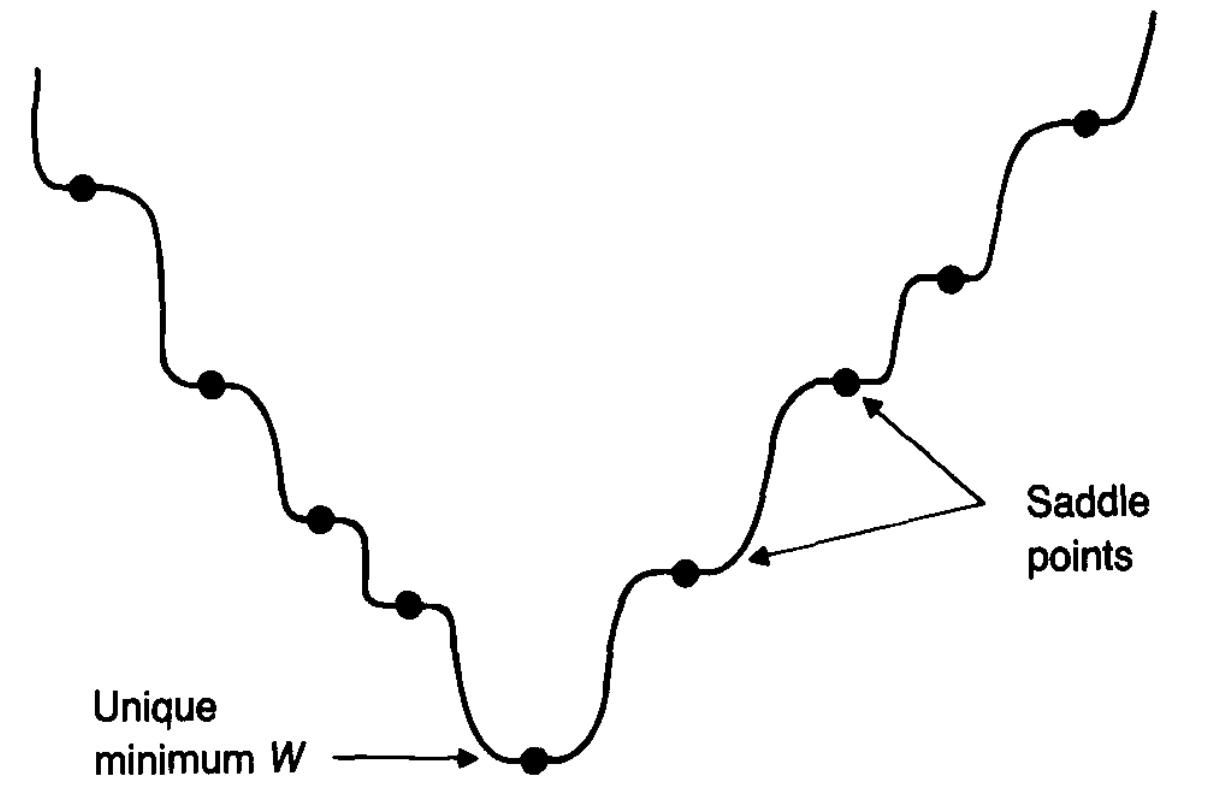
\includegraphics[width=0.4\textwidth]{./Images/LinearAutoenc_Saddles.png}
            \end{figure}
        \end{center}
        \newcolumn
        \begin{itemize}
            \item $\Sigma$ is full-rank with $n$ distinct eigenvalues $\lambda_1 > \dots > \lambda_n$
            \item $\mathcal{I} = {i_1, \dots, i_p}$ ($1 \leq i_1 < \dots < i_p \leq n$) is any ordered $p$-index set
            \item $U_{\mathcal{I}} = [ u_{i_1}, \dots, u_{i_p} ]$ matrix formed by the orthonormal eigenvectors of $\Sigma$ associated with the eigenvalues $\lambda_{i_1}, \dots, \lambda_{i_p}$
        \end{itemize}
    \end{multicols}
The critical map $W$ associated with the index set $\{1,2,\dots, p\}$ is the unique local and global minimum of $E$. The remaining $\binom{n}{p} - 1$ $p$-index sets correspond to saddle points. All additional critical points defined by matrices $A$ and $B$ which are not full rank are also saddle points and can be characterized in terms of orthogonal projections onto subspaces spanned by $q$ eigenvectors of $\Sigma$ with $q < p$
\end{frame}

\begin{frame}{Linear autoencoders}
Since we are applying only linear transformations, the best compression we can achieve is the one that projects the input data on the subspace spanned by the eigenvectors of the covariance matrix of the input data.\\
\vspace{1cm}
This corresponds to the \textbf{Principal Component Analysis (PCA)} when the input is normalized as follows:
\[
    \hat{x}_{i,j} = \dfrac{1}{\sqrt{m}}\left(x_{ij} - \dfrac{1}{m}\sum_{k=1}^m x_{kj}\right)
\]      
\end{frame}


\begin{frame}{Linear autoencoders}
    The aim is to minimize the recontruction error, i.e. the difference between the input data and the output data which can be written as:
    \[
        \min_{\theta} \sum_{i=1}^m \sum_{j=1}^n (x_{ij} - \hat{x}_{ij})^2 \hspace{0.3cm} \equiv \hspace{0.3cm} \min_{HW^*} (\|X - HW^*\|_F)^2
    \]
    From the Eckart-Young theorem, we know that the optimal solution is the truncated SVD:
\[
    HW^* = U_{:,\leq k}\Sigma_{k,k}V_{:,\leq k}^\intercal
\]
By matching variables one possible solution is:
\[
    H = U_{:,\leq k}\Sigma_{k,k} \hspace{0.5cm} W^* = V_{:,\leq k}^\intercal
\]
\end{frame}


\begin{frame}{Linear autoencoders}
\begin{proof}
    \begin{align*}
        H &= U_{:,\leq k}\Sigma_{k,k} \\
        &= (XX^T)(XX^T)^{-1}U_{:,\leq K}\Sigma_{k,k} \\
        &= (XV\Sigma^T U^T)(U\Sigma V^T V\Sigma^T U^T)^{-1}U_{:,\leq k}\Sigma_{k,k} \\
        &= XV\Sigma^T U^T(U\Sigma\Sigma^T U^T)^{-1}U_{:,\leq k}\Sigma_{k,k} \\
        &= XV\Sigma^T U^T U(\Sigma\Sigma^T)^{-1}U^T U_{:,\leq k}\Sigma_{k,k} \\
        &= XV\Sigma^T (\Sigma\Sigma^T)^{-1}U^T U_{:,\leq k}\Sigma_{k,k} \\
        &= XV\Sigma^T \Sigma^{T^{-1}}\Sigma^{-1}U^T U_{:,\leq k}\Sigma_{k,k}\\
        &= XV\Sigma^{-1} I_{:,\leq k}\Sigma_{k,k}\\
        &= XV I_{:,\leq k} = XV_{:,\leq k}
        \end{align*}
    
        Thus $H$ is a linear transformation of $X$ and the encoder matrix is the matrix of the first $k$ eigenvectors of the data covariance matrix. 
\end{proof}
\end{frame}


\section{Boolean autoencoders}
\begin{frame}{Boolean autoencoders}
    In the case of \textbf{Boolean autoencoders} we have:
    \begin{itemize}
        \item $\mathbb{F},\mathbb{G}$ are the Boolean fields, i.e $\{0,1\}$, the Galois field $\mathbb{F}_2$
        \item $\mathcal{A},\mathcal{B}$ are the classes of Boolean transformations: $A,B$ are unrestricted boolean functions
        \item $\Delta$ is the Hamming distance
    \end{itemize}
\end{frame}

\begin{frame}{Boolean autoencoders}
We start defining the following lemma:
\begin{lemma}
    The vector \text{Majority}(p) is a vector in $\mathbb{H}^n$ closest to the center of gravity of the vectors $p_1, \dots, p_k$ and it minimizes the function $E(q) = \sum_{i=1}^k \Delta(p_i, q)$.
\end{lemma}
Where the center of gravity is the vector $c$ in $\mathbb{R}^n$ with coordinates 
\[
    c_j = \dfrac{\left(\sum\limits_{i=1}^{k} p_{ji}\right)}{k}
\]
So, each $c_j$ is the average of the $j$-th components of the vectors $p_1, \dots, p_k$.
For any $j$, $(p)_j$ is the closest binary value to $c_j$.
\end{frame}



\begin{frame}{Boolean autoencoders}
This means that for each row, we check the majority of the values and we set the value of the row to the majority value.\\
\vspace{1cm}
\[
    n\text{ rows }
  \begin{bmatrix}
    \flag{left}{1} & 0  & 1 & 1 & 1 & \flag{right}{0}\\
    0 & 0 & 1 & 1 & 0 & 0 \\
    1 & 1 & 0 & 1 & 1 & 0 \\
    1 & 0 & 1 & 0 & 1 & 0 \\
    0 & 1 & 1 & 1 & 0 & 1 \\
    0 & 0 & 0 & 0 & 0 & 1 \\
    0 & 1 & 0 & 0 & 0 & 1 \\
    0 & 0 & 0 & 1 & 0 & 0 \\
  \end{bmatrix}
  \hspace{3cm}
  \highlight{N}
  \underbrace{\begin{bmatrix}
    \flag{left}{1}
    \flag{right}{}  \\
    0 \\
    1 \\
    0 \\
    1 \\
    0 \\
    0 \\
    0 \\
  \end{bmatrix}}_{\text{Majority}(p)}
  \highlight{NT}
  \in \mathbb{H}^n
\]
\overlay{
  \draw[->, thick, red, dashed] (N) -- (NT)
    node [pos=0.48, above] {$p_1$};
  \node[above of = N ] { $k$ column vectors   };
}

\end{frame}


\begin{frame}{Boolean autoencoders}
    A \textbf{Voronoi partition} of $\mathbb{H}^n$ generated by the vectors $p_1, \dots, p_k$ is a partition of $\mathbb{H}^n$ into $k$ regions $\mathcal{C}^{Vor}(p_1), \dots, \mathcal{C}^{Vor}(p_k)$ such that for each $x$ in $\mathbb{H}^n$:
\[
    x \in \mathcal{C}^{Vor}(p_i) \iff \Delta(x, p_i) \leq \Delta(x, p_j) \text{ for all } j \neq i    
\]
\begin{multicols}{2}
    \begin{center}
        \begin{figure}[H]
            \centering
            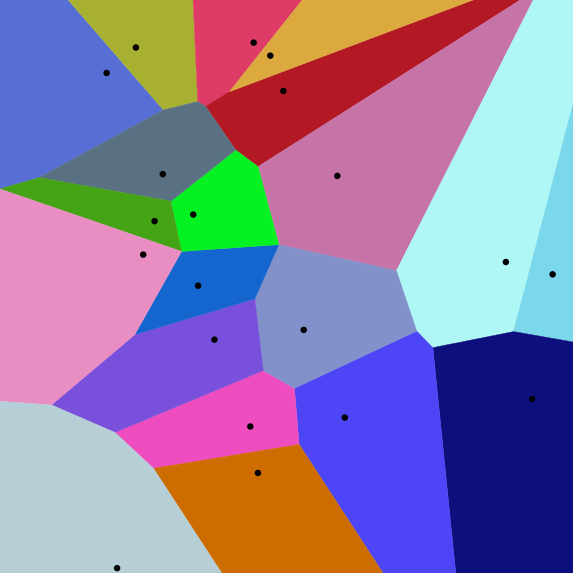
\includegraphics[width=0.3\textwidth]{./Images/Euclidean_Voronoi_diagram.png}
            \caption{Euclidean distance}
        \end{figure}
    \end{center}
    \begin{center}
        \begin{figure}[H]
            \centering
            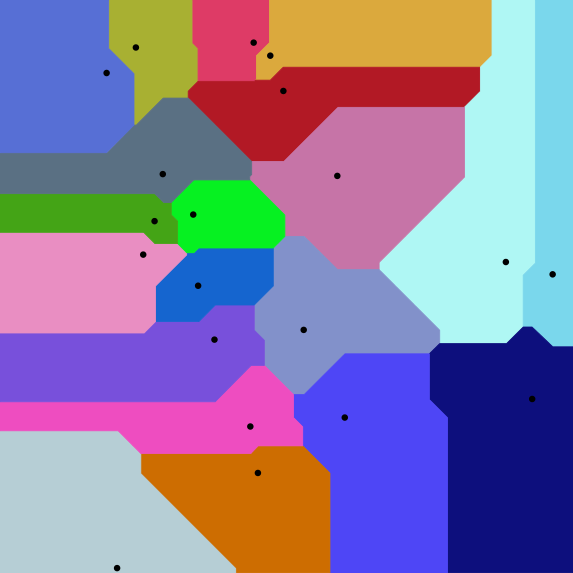
\includegraphics[width=0.3\textwidth]{./Images/Manhattan_Voronoi_Diagram.png}
            \caption{Manhattan distance}
        \end{figure}
    \end{center}
\end{multicols}
\end{frame}


\begin{frame}{Boolean autoencoders}
Considering the two steps mapping:
\[
    x \xrightarrow{B} h \xrightarrow{A} y
\]
Where the dimension of the hidden layer is $p$, so there are $2^p$ possible configurations of the hidden layer, denoted by $h_1, \dots, h_{2^p}$.
\hspace{0.5cm}
\begin{theorem}
    \textbf{Fixed layer solution}: if the $A$ mapping is fixed , then the optimal mapping $B^*$ is given by $B^*(x) = h_i$ for any $x$ in $\mathcal{C}_i = \mathcal{C}^{Vor}(A(h_i))$. Conversely, if $B$ is fixed, then the optimal mapping $A^*$ is given by $A^*(h_i) = \text{Majority}\left[\mathcal{X} \cap B^{-1}(h_i)\right]$ 
\end{theorem}
\end{frame}


\begin{frame}{Boolean autoencoders}
    \begin{multicols}{2}
        If we consider the input-output layers to have a cardinality of 4 and the hidden layer to have a cardinality of 2, then this would mean that there would be $2^2 = 4$ centroids given by the $A$ mapping in the space $\mathbb{H}^4$ showed in figure:

        \begin{figure}[H]
            \centering
            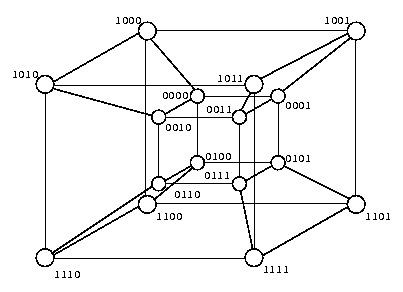
\includegraphics[width=0.4\textwidth]{./Images/Hypercube4Dimensions.png}
            %\caption{Hypercube in 4 dimensions}
        \end{figure}
    \end{multicols}
    So, the Voronoi partition would be the partition of the hypercube into 4 regions using as metric the Hamming distance, i.e. the number of edges that need to be crossed to go from one point to each centroid.

\end{frame}

\section{Clustering complexity}
\begin{frame}{Complexity recap}
The basic classes for complexity are:
\begin{itemize}
    \item $\mathcal{P}$ is the class of problems that can be \textit{solved} in polynomial time by a deterministic TM
    \item $\mathcal{NP}$ is the class of problems for which a solution can be \textit{verified} in polynomial time by a deterministic TM. The class $\mathcal{NP}$ is the class of problems that can be solved non-deterministically in polynomial time
    \begin{itemize}
        \item \textbf{$\mathcal{NP}$-complete} if it is in $\mathcal{NP}$ and every problem in $\mathcal{NP}$ can be reduced to it in polynomial time
        \item \textbf{$\mathcal{NP}$-hard} if there is a $\mathcal{NP}$-complete problem that can be reduced to it in polynomial time
    \end{itemize}
\end{itemize}
\end{frame}




\begin{frame}{Clustering complexity}
    \begin{theorem}
        Consider the following hypercube clustering problem:
        \begin{itemize}
            \item \textbf{Input:} $m$ binary vectors $x_1, \dots, x_m$ of length $n$ and an integer $k$
            \item \textbf{Output:} $k$ binary vectors $c_1, \dots, c_k$ of length $n$ (the centroids) and a function $f$ from $\{x_1, \dots, x_m\}$ to $\{c_1, \dots, c_k\}$ that minimizes the distortion 
            \[
                E = \sum_{t=1}^m \Delta(x_t, f(x_t))    
            \]
            Where $\Delta$ is Hamming distance.
        \end{itemize}
        The hypercube clustering decision problem $\mathcal{NP}$-hard when $k \sim m^\epsilon$ $(\epsilon > 0)$
    \end{theorem}
\end{frame}



\begin{frame}{Clustering complexity}
To prove the hypercube clustering problem is $\mathcal{NP}$-hard we need to demonstrate that an $\mathcal{NP}$-complete problem can be reduced to it in polynomial time. The following reductions are used:
\begin{center}
    \smartdiagram[flow diagram:horizontal]{3-SAT, $\mathbb{R}^2$ clustering, hypercube\ clustering}
\end{center}
\vspace{0.3cm}
To sketch the reduction, we start from the problem of clustering $m$ points in the plane $\mathbb{R}^2$ using cluster centroids and the $L_1$ distance, which is $\mathcal{NP}$-complete by reduction from 3-SAT when $k \sim m^\epsilon$ $(\epsilon > 0)$. Without any loss of generality, we can assume that the points in these problems lie on the vertices of a square lattice. Using the theorem in Havel and Moràvek paper, one can show that a $n \times m$ square lattice in the plane can be embedded in a hypercube $\mathbb{H}^{m+n}$.    
\end{frame}


\begin{frame}{Clustering complexity}

    Example:
    \begin{multicols}{2}
    \begin{center}
                % 4x2 Lattice with different shaped lines
        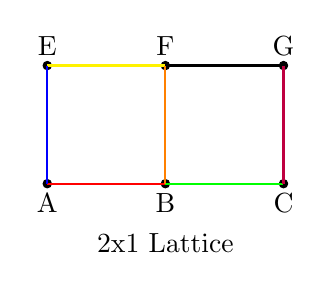
\begin{tikzpicture}[scale=1.5]
            % Draw the grid points
            \filldraw[black] (0,0) circle (1pt) node[anchor=north] {A};
            \filldraw[black] (1,0) circle (1pt) node[anchor=north] {B};
            \filldraw[black] (2,0) circle (1pt) node[anchor=north] {C};
            %\filldraw[black] (3,0) circle (1pt) node[anchor=north] {D};

            \filldraw[black] (0,1) circle (1pt) node[anchor=south] {E};
            \filldraw[black] (1,1) circle (1pt) node[anchor=south] {F};
            \filldraw[black] (2,1) circle (1pt) node[anchor=south] {G};
            %\filldraw[black] (3,1) circle (1pt) node[anchor=south] {H};

            % Connect the points with different line styles
            \draw[red,thick] (0,0) -- (1,0); % Solid line
            \draw[green,thick] (1,0) -- (2,0); % Dashed line
            %\draw[dotted, thick] (2,0) -- (3,0); % Dotted line
            \draw[yellow,thick] (0,1) -- (1,1); % Dash-dot line
            \draw[thick] (1,1) -- (2,1); % Solid line
            %\draw[dashed, thick] (2,1) -- (3,1); % Dashed line
            \draw[blue,thick] (0,0) -- (0,1); % Dotted line
            \draw[orange,thick] (1,0) -- (1,1); % Dash-dot line
            \draw[purple,thick] (2,0) -- (2,1); % Solid line
            %\draw[dashed, thick] (3,0) -- (3,1); % Dashed line

            % Label the lattice
            \node at (1, -0.5) {2x1 Lattice};
        \end{tikzpicture}
    \end{center}
    \columnbreak
    \begin{center}
                % 3D Cube with connections following the lattice pattern
        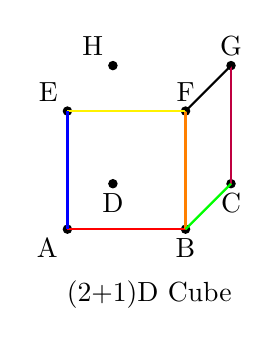
\begin{tikzpicture}[scale=1.5]
            % Draw the vertices of the cube (front and back face)
            \filldraw[black] (0,0,0) circle (1pt) node[anchor=north] {D}; % Front bottom left
            \filldraw[black] (1,0,0) circle (1pt) node[anchor=north] {C}; % Front bottom right
            \filldraw[black] (0,1,0) circle (1pt) node[anchor=south east] {H}; % Front top left
            \filldraw[black] (1,1,0) circle (1pt) node[anchor=south] {G}; % Front top right

            \filldraw[black] (0,0,1) circle (1pt) node[anchor=north east] {A}; % Back bottom left
            \filldraw[black] (1,0,1) circle (1pt) node[anchor=north] {B}; % Back bottom right
            \filldraw[black] (0,1,1) circle (1pt) node[anchor=south east] {E}; % Back top left
            \filldraw[black] (1,1,1) circle (1pt) node[anchor=south] {F}; % Back top right

            % Connect the vertices with corresponding line styles from the lattice
            %\draw[green,thick] (0,0,0) -- (1,0,0); % Solid line (A-B)
            \draw[purple,thick] (1,0,0) -- (1,1,0); % Dashed line (B-F)
            %\draw[purple,thick] (0,1,0) -- (1,1,0); % Dotted line (E-F)
            %\draw[green,thick] (0,0,0) -- (0,1,0); % Dash-dot line (A-E)

            \draw[red,thick] (0,0,1) -- (1,0,1); % Solid line (C-D)
            \draw[orange,thick] (1,0,1) -- (1,1,1); % Dashed line (D-H)
            \draw[yellow,thick] (0,1,1) -- (1,1,1); % Dotted line (G-H)
            \draw[blue,thick] (0,0,1) -- (0,1,1); % Dash-dot line (C-G)

            % Connect the front and back face vertices
            %\draw[blue,thick] (0,0,0) -- (0,0,1); % Solid line (A-C)
            \draw[green,thick] (1,0,0) -- (1,0,1); % Dashed line (B-D)
            %\draw[blue,thick] (0,1,0) -- (0,1,1); % Dotted line (E-G)
            \draw[,thick] (1,1,0) -- (1,1,1); % Dash-dot line (F-H)

            % Label the cube
            \node at (0.5, -0.75, 0.5) {(2+1)D Cube};
        \end{tikzpicture}        
    \end{center}

        \end{multicols}
        It is easy to check that the $L_1$ or Manhattan distance between any two points on the square lattice is equal to the corresponding Hamming distance in $\mathbb{H}^{m+n}$.
        This polynomial reduction completes the proof that if the number of cluster satisfies $k = 2^p \sim m^\epsilon$ or equivalently $p \sim \epsilon \log_2 m \sim C \log n$, then the hypercube clustering problem associated with the Boolean autoencoder is $\mathcal{NP}$-hard and the corresponding decision problem is $\mathcal{NP}$-complete.
\end{frame}



\begin{frame}
    \begin{center}
        \Huge
        Thank you for your attention!
    \end{center}
\end{frame}

\end{document}
